\chapter{実験方法とその結果}
\label{chap:ledoxea}

本章では、開発したスマートフォンアプリDreamtravelerの実験方法(調査対象・観察方法)と実験結果のについて説明する。

\section{実験方法}
 外的刺激が夢に影響を与えるか否かを調べるために15日間の実験に参加してもらった。実験を通して何も音楽を流さない場合と流した場合の結果の違いを分析した。15日間という実験記録を集めたのは、睡眠に関する実験は体調、その日の活動内容や、被験者の心境によって左右されがちでデーターが変動しやすいためである。\\
 そうすることで夢を記憶できる体質になってもらうことを目指した。またスマートフォンは充電をした状態で枕の横に置いてもらうことで、音声が脳に届く状態にしてもらった。\\
 実験は1日目は音楽なし、2日目はREM睡眠中音楽あり、3日目は起きる直前のREM睡眠中音楽ありというを繰り返し5回、合計15日間続けてもらった。被験者にはThe MILD Techniqueに基づいて夢を記憶できる体質になってもらうために実験を開始する5〜10日間前から、被験者には夢日記を書いてもらった。加えて、寝る前に音楽を聴きながら思い出に関する画像を2分間眺めること、思い出について考えならが寝る意識をしてもらった。また6時間以上睡眠を取れる日にのみ実験に臨んでもらった。詳しい事件内容は以下に述べる。

\section{実験スケジュール}
図\ref{schedule}これが実験のスケジュールである。(※この内容は付録に回すかも)
\begin{figure}[htbp]
\begin{center}
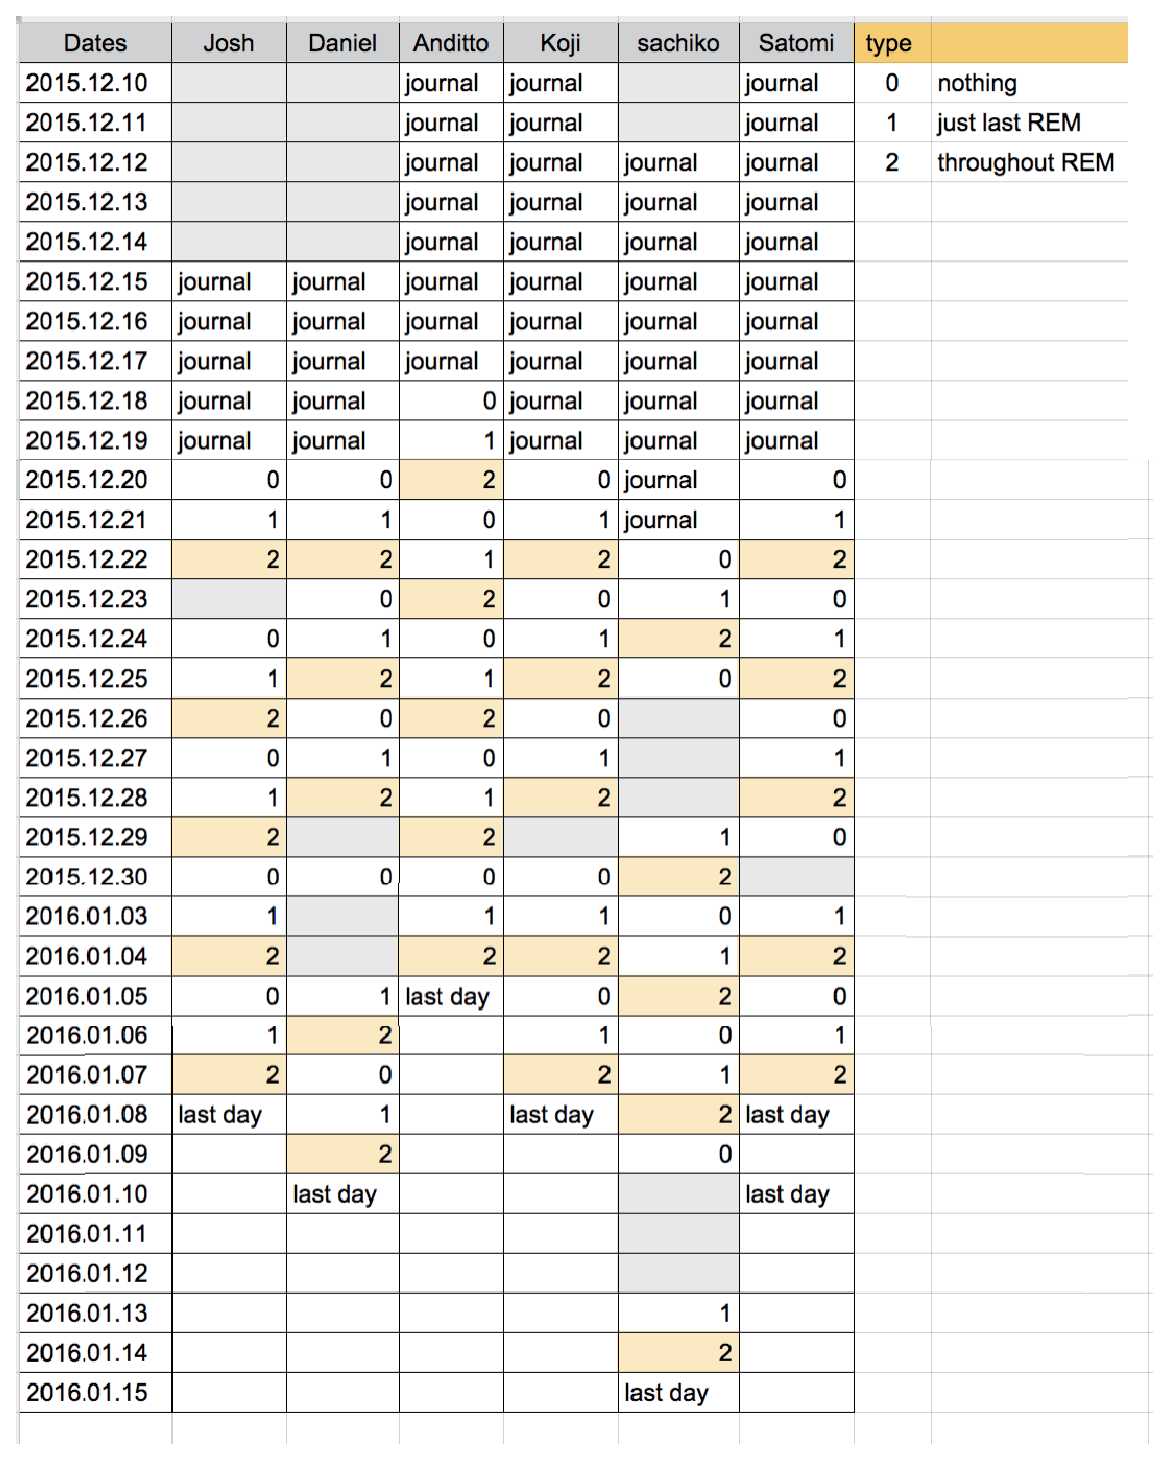
\includegraphics[width=15cm]{eps/schedule.eps}
\caption{Dreamtraveler実験スケジュール}
\label{schedule}
\end{center}
\end{figure}

\section{調査対象}
20歳〜50歳の男女5人に参加してもらった。5人の被験者は皆明晰夢に興味がある人。一人は普段から経験している人。一人は一度もしたことない人。音にどれくらい敏感かも述べる。比較的一定の睡眠活動をしている人を対象にした。

被験者1:
\begin{itemize}
\item 国籍:インドネシア人
\item 性別:男性
\item 年齢:30代後半
\item 明晰夢の経験:5回ほど経験している
\item 夢日記を行ったか否か:5日間行った
\item 思い出に由来する音楽:コーヒーを飲むときに決まって聴く曲
\end{itemize}

被験者2:
\begin{itemize}
\item 国籍:日本人
\item 性別:女性
\item 年齢:40代後半
\item 明晰夢の経験:経験したことなし
\item 夢日記を行ったか否か:10日間行った
\item 思い出に由来する音楽:結婚式で流れた曲
\end{itemize}

被験者3:
\begin{itemize}
\item 国籍:日本人
\item 性別:男性
\item 年齢:50代前半
\item 明晰夢の経験:経験したことなし
\item 夢日記を行ったか否か:10日間行った
\item 思い出に由来する音楽:007映画で出演者になりたい
\end{itemize}

被験者4:
\begin{itemize}
\item 国籍:アメリカ人
\item 性別:男性
\item 年齢:20代前半
\item 明晰夢の経験:5回以上経験したことがある
\item 夢日記を行ったか否か:5日間ほど行った
\item 思い出に由来する音楽:ジブリの映画
\end{itemize}

被験者5:
\begin{itemize}
\item 国籍:日本人
\item 性別:女性
\item 年齢:20代後半
\item 明晰夢の経験:経験したことない
\item 夢日記を行ったか否か:5日間ほど行った
\item 思い出に由来する音楽:ダンスで起用した曲
\end{itemize}


被験者6:
\begin{itemize}
\item 国籍:アメリカ人
\item 性別:男性
\item 年齢:20代前半
\item 明晰夢の経験:何度か経験したことがある
\item 夢日記を行ったか否か:5日間行った
\item 思い出に由来する音楽:高校時代で組んでたバンドの音楽
\end{itemize}

被験者7:
\begin{itemize}
\item 国籍:アメリカ人
\item 性別:男性
\item 年齢:20代後半
\item 明晰夢の経験:5回以上経験したことある
\item 夢日記を行ったか否か:5日間ほど行った
\item 思い出に由来する音楽:彼女に作った音楽
\end{itemize}

\section{観察の方法}

\section{実験結果}
図\ref{experiment}に実験結果を合わせて表示する。
\begin{figure}[htbp]
\begin{center}
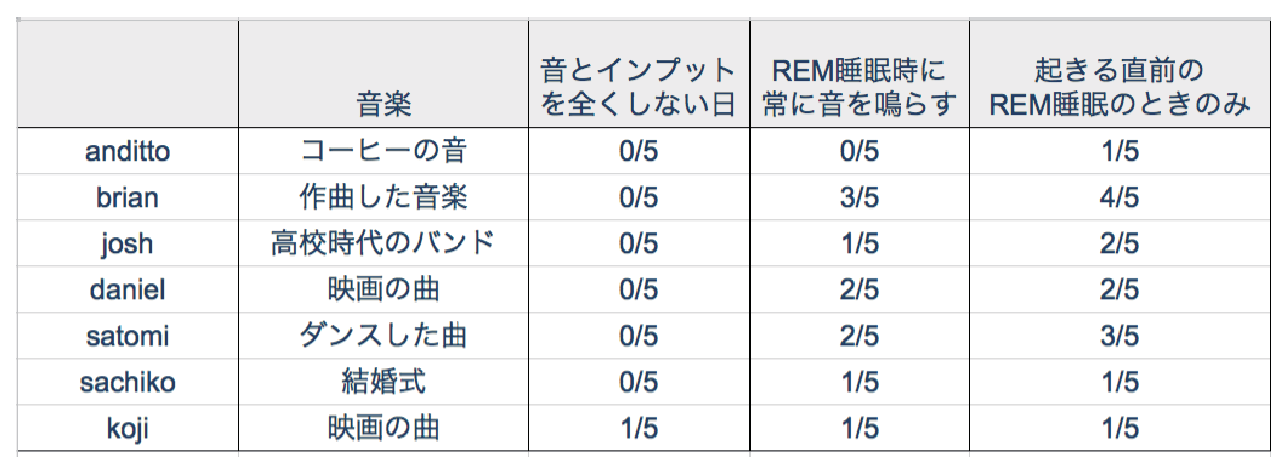
\includegraphics[width=15cm]{eps/eperiment.eps}
\caption{Dreamtraveler:実験結果}
\label{experiment}
\end{center}
\end{figure}

\subsection{より詳しい実験結果}

\begin{itemize}
\item 被験者1:音楽を普段から聞かない人に生活習慣の中に特定の音を組み入れたもらった結果\\
 被験者1は音楽にあまり関心がなく、特に思い出に残る音・音楽がなかった。被験者1は世界中の豆を集めるほどの大のコーヒー好きということだった。そこで実験10日間前から毎日コーヒーを飲むときにEdith Piafによる"Non je ne regrette rien"という曲を聴いてもらうようにした。こうすることで体験と特定の音を紐付けることを試みた。この音楽は映画inceptionの中で夢から覚めるために主人公たちが聴く音楽としても知られている。すると音のインプットしない日は一度も関連する夢は見なかったが、起きる直前のREM睡眠のときに、コーヒーを飲む夢を見ることに成功した。

\item 被験者2:夢を見たい記憶が昔である場合:\\
 被験者2は30年ほど前の結婚式の夢を見ることを望んだ。そこで結婚式で流した音楽 The CarpentersによるWe've only just begunを実験で扱うことにした。するとREM睡眠時に常に音楽を鳴らした3日目と起きる直前のREM睡眠時に音楽を鳴らした5日目に結婚式当初の夢を見ることに成功した。

\item 被験者3と被験者4:見たい夢が、実体験の経験ではなく視聴した映画なぞの映像だった場合:\\
 被験者3は007の映画、被験者4は宮崎駿の映画である「魔女の宅急便キキ」の映画を体験したいということだった。そこでそれぞれの曲で使われている音楽を起用した。すると被験者3はインプットしない日の5日目、REM睡眠時に常に音を鳴らした日の5日目、起きる直前のREM睡眠のの5日目にそれぞれ一回ずつ007の夢を見た。すべて実験終盤の結果である。\\
 被験者4はインプットしない日は全く夢を見なかったことに対して、REM睡眠時に常に音を鳴らした日は2/5の確率で夢を見た。そして起きる直前のREM睡眠時は3/5の確率で夢を見たのだ。

\item 被験者5と被験者6と被験者7:自分で作曲・演奏・演出した音楽である場合:\\
 被験者5は今年の9月に社会人ダンス部でダンスを披露したときに起用した曲、被験者6は高校時代にバンドで演奏した曲、被験者7は今年の11月に自らが交際相手のために作曲・演奏した曲を起用した。\\
 被験者5はインプットを全くしない日は関連した夢を見なかったのに対して、REM睡眠時に常に音を鳴らしたときに1/5の確率でダンスの夢を、起きる直前のREM睡眠のときのみ音を流したときは1/5の確率で関連する夢を見た。\\
 被験者6はインプットを全くしない日は関連した夢を見なかったのに対して、REM睡眠時に常に音を鳴らしたときに1/5の確率でバンド時代の夢を、起きる直前のREM睡眠のときのみ音を流したときは2/5の確率で関連する夢を見た。\\
 被験者6はインプットを全くしない日は関連した夢を見なかったのに対して、REM睡眠時に常に音を鳴らしたときに3/5の確率でバンド時代の夢を、起きる直前のREM睡眠のときのみ音を流したときは4/5の確率で関連する夢を見た。
\end{itemize}

\section{解析結果の考察}
 以上の実験結果から、下記の点が分かった。

\subsection{音の効果、有効的なタイミング}
 インプットを全くしない日に夢を見たのは1/35の確率だったのに対し、REM睡眠時に常に音を鳴らしたときは9/35の確率であった。そして起きる直前のREM睡眠のときのみ音を流したときは13/35であった。これらの結果から音による刺激は夢に対してなんらかの操作がかかっているということが示された。またREM睡眠時に常に音を流すのと起きる直前のREM睡眠のときのみ音を流すのでは、直前のみに音を流す方が高い効果が見れた。

\subsection{Dreamtravelerを長く使用すれば使用するほど効果が高まる}

\subsection{睡眠に入る前に瞑想をする時間、写真を眺める時間を加えた方が高い効果が見込まれる}

\subsection{年齢層が高いほど影響を受けにくい可能性がある}